\subsection{Remove border blobs}

Op het moment dat er een beeld binnen komt beschouwen we rand objecten als
nutteloos. Simpelweg omdat het niet zeker is wat het voor object is. Daarom
wordt er gebruik gemaakt van de \emph{remove border blobs} operatie.

Er komt een binair plaatje binnen bestaande uit 1-en en 0-en. Door de 1-en
aan de rand van het plaatje te markeren met een ander nummer kan er een
border blob geïdentificeerd worden.

Omdat enkel de rand gescand hoeft te worden kan deze functie redelijk snel
uitgevoerd worden (listing \ref{lst:border-marking}).

Het voltooien van het markeren is mogelijk door, als er een 1 gezien wordt,
te kijken naar de buren van deze pixel. Als dat een 2 is, dan mag deze pixel
ook gemarkeerd worden als een 2 enzovoort. Dit markeren kan van rechts-onder
naar links-boven en van links-boven naar rechts-onder gedaan worden om het
aantal iteraties te verminderen. Door iedere keer na een markeer ronde te
controleren of er een 1-2 verbinding bij X-connected is, kan er bepaald worden
of er nog een keer over het plaatje gegaan moet worden om de overige pixels te
markeren (figuur \ref{fig:bbstep2}). De scan van links boven naar rechts onder
en van rechts onder naar rechts boven kan in een loop uitgevoerd worden (listing
\ref{lst:mark-border-neighbours}). Tot slot kan er dan met een functie alle
pixels met een 2 markeren als een 0 (figuur \ref{fig:bbstep3}).


\begin{listing}
    \begin{minted}{c}
        for (x = FRAME_WIDTH; x > 0; x--){
            dst->data[0][(x - 1)]            = dst->data[0][(x - 1)] * 2;
            dst->data[FRAME_HEIGHT][(x - 1)] = dst->data[FRAME_HEIGHT][(x - 1)] * 2;
        }

        for (y = FRAME_HEIGHT; y > 0; y--) {
            dst->data[(y - 1)][0]            = dst->data[(y - 1)][0] * 2;
            dst->data[(y - 1)][FRAME_WIDTH]  = dst->data[(y - 1)][FRAME_WIDTH] * 2;
        }
    \end{minted}
    \caption{Markeren rand pixels die onderdeel zijn van een blob}
    \label{lst:border-marking}
\end{listing}

\begin{figure}
    \begin{center}
        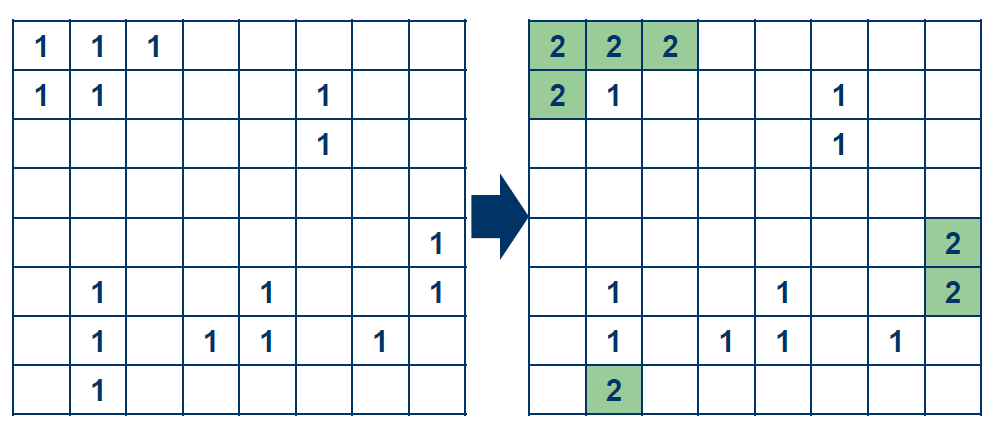
\includegraphics[scale=0.35]{figures/border_blob_step1.png}
    \end{center}
    \caption{Rand blobs markeren}
    \label{fig:bbstep1}
\end{figure}

\begin{figure}
    \begin{center}
        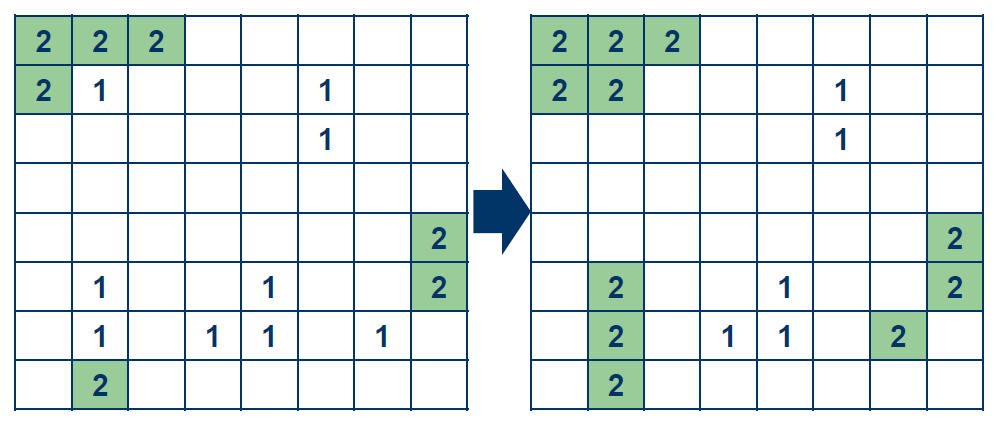
\includegraphics[scale=0.35]{figures/border_blob_step2.png}
    \end{center}
    \caption{Blijf scannen en markeren tot alles is gemarkeerd}
    \label{fig:bbstep2}
\end{figure}

\begin{listing}
    \begin{minted}{c}
        // Lower right to top left
        if(img[i] == 1){
            if(iNeighbourCount(img, w, h, 2, connected) > 0){
                img[i] = 2;
            }
        }

        // Top left to lower right
        if(img[size - i] == 1){
            if(iNeighbourCount(img, (width - w), (height - h), 2, connected) > 0){
                img[size - i] = 2;
            }
        }
    \end{minted}
    \caption{Scannen van alle rand blobs}
    \label{lst:mark-border-neighbours}
\end{listing}

\begin{figure}
    \begin{center}
        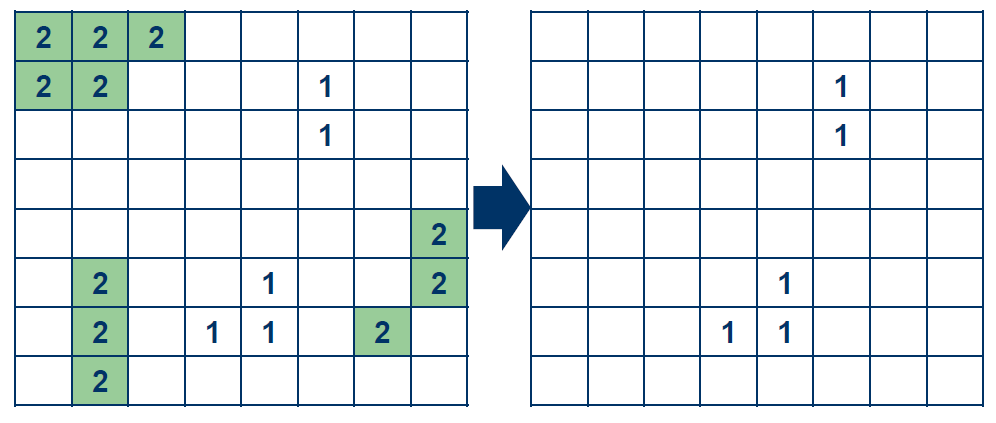
\includegraphics[scale=0.35]{figures/border_blob_step3.png}
    \end{center}
    \caption{Maak alle pixels gemarkeerd met 2 naar 0}
    \label{fig:bbstep3}
\end{figure}
